\documentclass[
    %aspectratio=169,
]{beamer}

\usepackage[english]{babel}
\usepackage[utf8]{inputenc}
\usepackage[T1]{fontenc}
\usepackage{csquotes}
\usepackage{expl3,biblatex}

\addbibresource{bibliography.bib}

\usepackage{booktabs}
\usetheme{Madrid}
\usecolortheme{crane}
\usepackage{svg}
\usepackage{graphicx,caption}

% set font
\usefonttheme{serif}

% to prevent the boxes from overlapping the logo at the lower right corner
\addtobeamertemplate{block begin}{%
  \setlength{\textwidth}{0.9\textwidth}%
}{}

\addtobeamertemplate{block alerted begin}{%
  \setlength{\textwidth}{0.9\textwidth}%
}{}

\addtobeamertemplate{block example begin}{%
  \setlength{\textwidth}{0.9\textwidth}%
}{}


% usage: \hl{text to emphasis as yellow background}
\usepackage{soul}
\makeatletter
\let\HL\hl
\renewcommand\hl{%
  \let\set@color\beamerorig@set@color
  \let\reset@color\beamerorig@reset@color
  \HL}
\makeatother


% usage: create outline pages before each section
\AtBeginSection[]
{
  \begin{frame}
    \frametitle{Table of Contents}
    \tableofcontents[currentsection]
  \end{frame}
}

\setbeamertemplate{caption}[numbered]

% Title page information
\title[Using LLMs for Translationese]{Using Large Language Models in Translationese Classification}
\author[Dani Baciu]{Student: Baciu Daniel Mihai\texorpdfstring{\\}{, }Scientific Coordinator: Lect. Dr. Bogdan Dumitru}
\institute[UniBuc]{University of Bucharest}
\date{\today}
\subject{Presentation Subject}
\keywords{the, presentation, keywords}

\begin{document}

% make the title page
\begin{frame}%[plain]
\maketitle
\end{frame}

% make the outline page/table of contents
% \begin{frame}
% \frametitle{Table of Contents}
% \tableofcontents
% \end{frame}






\section[The problem addressed]{The problem addressed}

\begin{frame}{The problem addressed}

\hspace{0.4cm} The need to improve translationese classification and the potential of large language models (LLMs) to enhance translation detection accuracy. 
\vspace{1cm}
\begin{block}{}
As two languages can not be perfectly mapped with each other $\rightarrow$ translated text and its original can not be perfectly matched.
\end{block}

\end{frame}







\section[The proposed solution]{The proposed solution}

\begin{frame}{The proposed solution}

\hspace{0.4cm} In the process of obtaining the best accuracy, I initially passed all the texts through the BERT model which was set in test mode, that is, backward() was not done through the network. Then I trained several Neural Networks (NN) to see which ones presented the best accuracy. The best models from Experiment 1 were used further, in Experiment 2.

\end{frame}






\section[Technologies used]{Technologies used}

\begin{frame}{Technologies used}

Technologies used:
\begin{itemize}
    \item Python
    \item PyTorch
    \item BERT
    \item Hugging Face
\end{itemize}

\end{frame}










\section[Dataset]{Dataset}

\begin{frame}{Dataset}

\begin{center}
    \begin{figure}[!h]
        \centering
        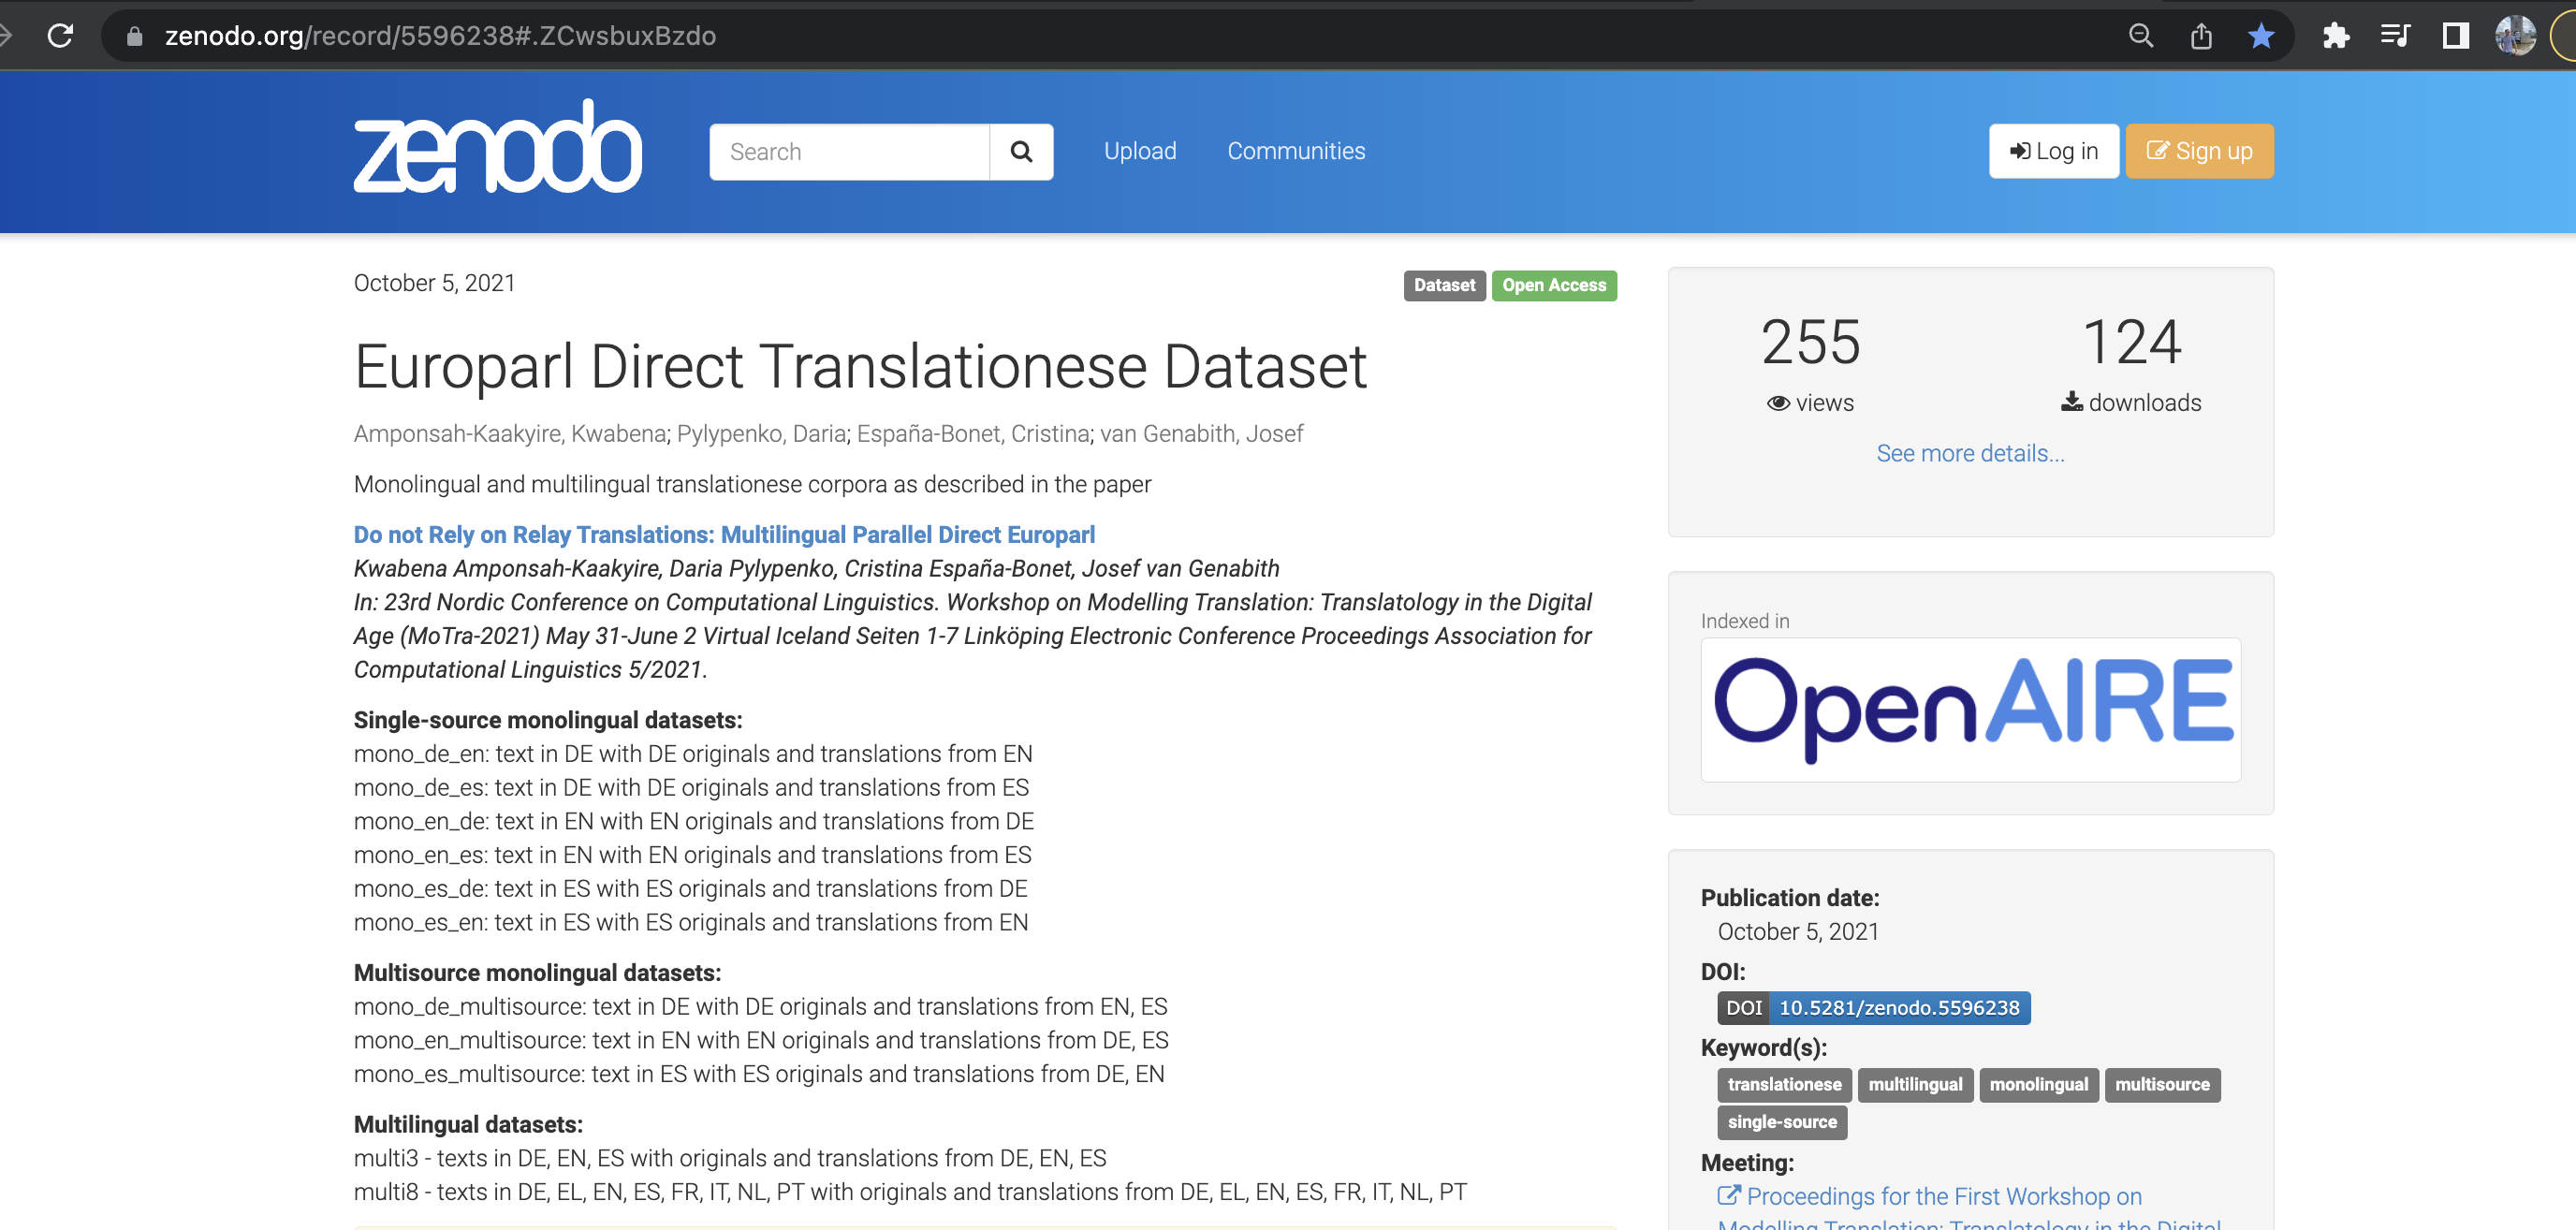
\includegraphics[width=\textwidth]{img/dataset-zenodo.png}
        \label{fig:dataset1}
        \caption{Europarl Direct Translationese Dataset}
    \end{figure}
\end{center}

\end{frame}



\begin{frame}{Dataset}

\begin{center}
    \begin{figure}[!h]
        \centering
        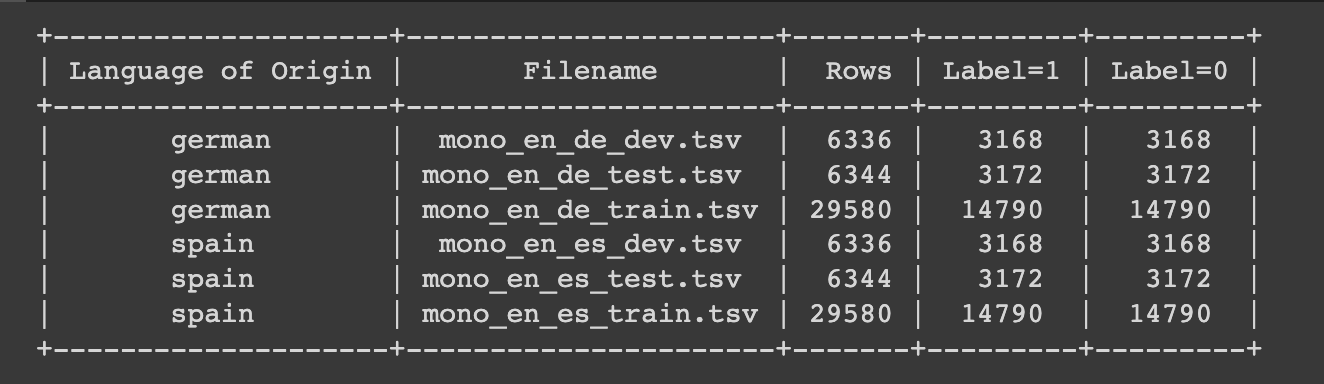
\includegraphics[width=\textwidth]{img/dataset.png}
        \label{fig:dataset}
        \caption{Dataset}
    \end{figure}
\end{center}

\end{frame}








\section[Technical implementation]{Technical implementation}

\begin{frame}{Technical implementation}{Experiment 1}

\hspace{0.4cm} Experiment 1 consisted of finding the best model for fine-tuning. The tested models exhibited variations in both the type and quantity of layers employed, as well as various activation functions. The number of epochs was the same for all, this being 50. The learning rate took values from the following array 
$[4*10^{-5}, 4*10^{-4}, 2*10^{-4}, 10^{-4},$ \newline $6*10^{-3}, 4*10^{-3}, 2*10^{-3}, 10^{-3}]$. The batch size remained constant at 32.

\end{frame}

\begin{frame}{Technical implementation}{Experiment 1}

\begin{center}
    \begin{figure}[!h]
        \centering
        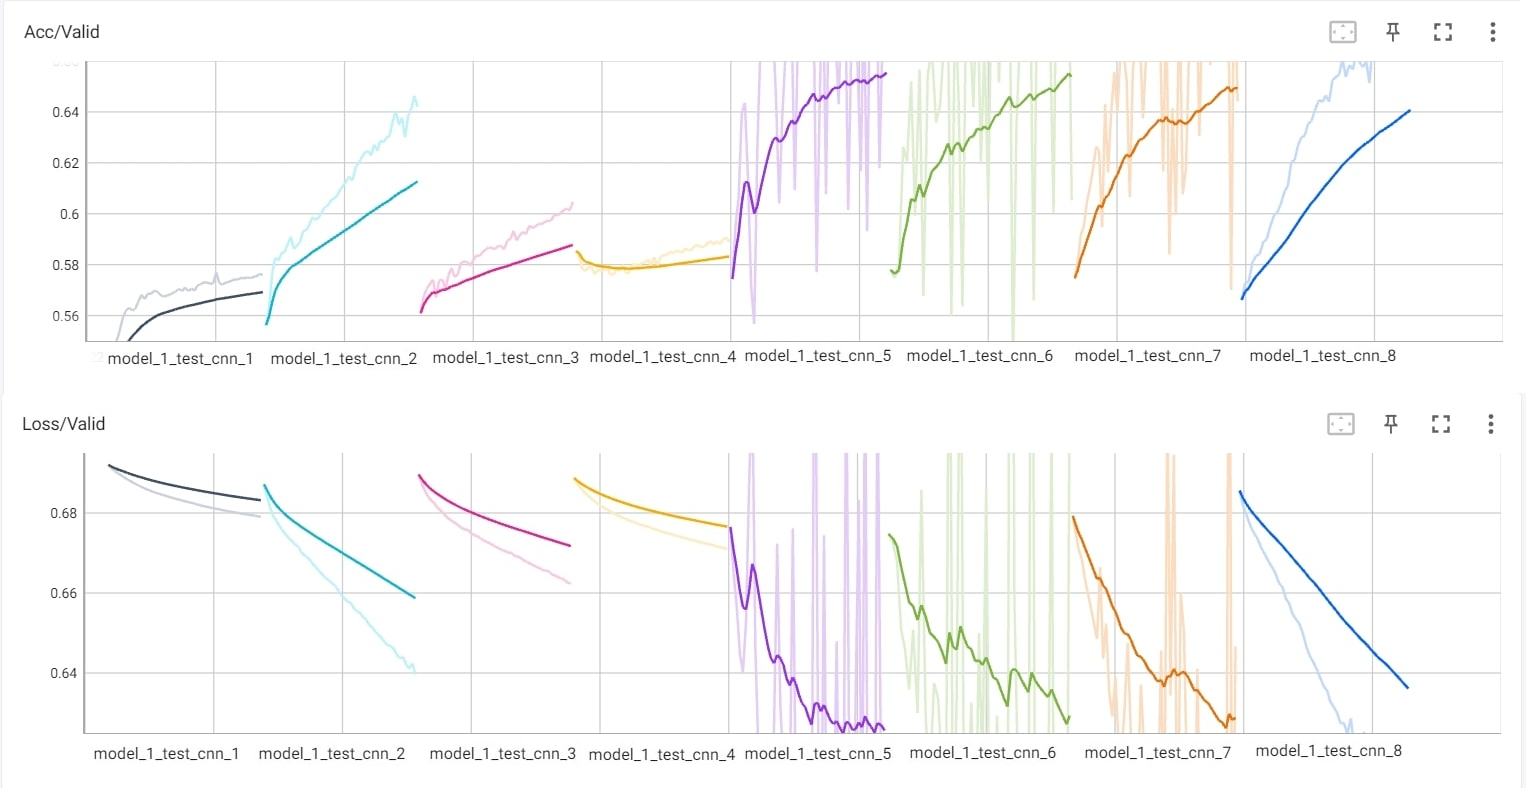
\includegraphics[width=\textwidth]{img/exp1_acc1+loss1.jpg}
        \label{fig:exp1_mod1}
        \caption{Experiment 1 - Results for Model 1}
    \end{figure}
\end{center}

\end{frame}


\begin{frame}{Technical implementation}{Experiment 1}

\begin{center}
    \begin{figure}[!h]
        \centering
        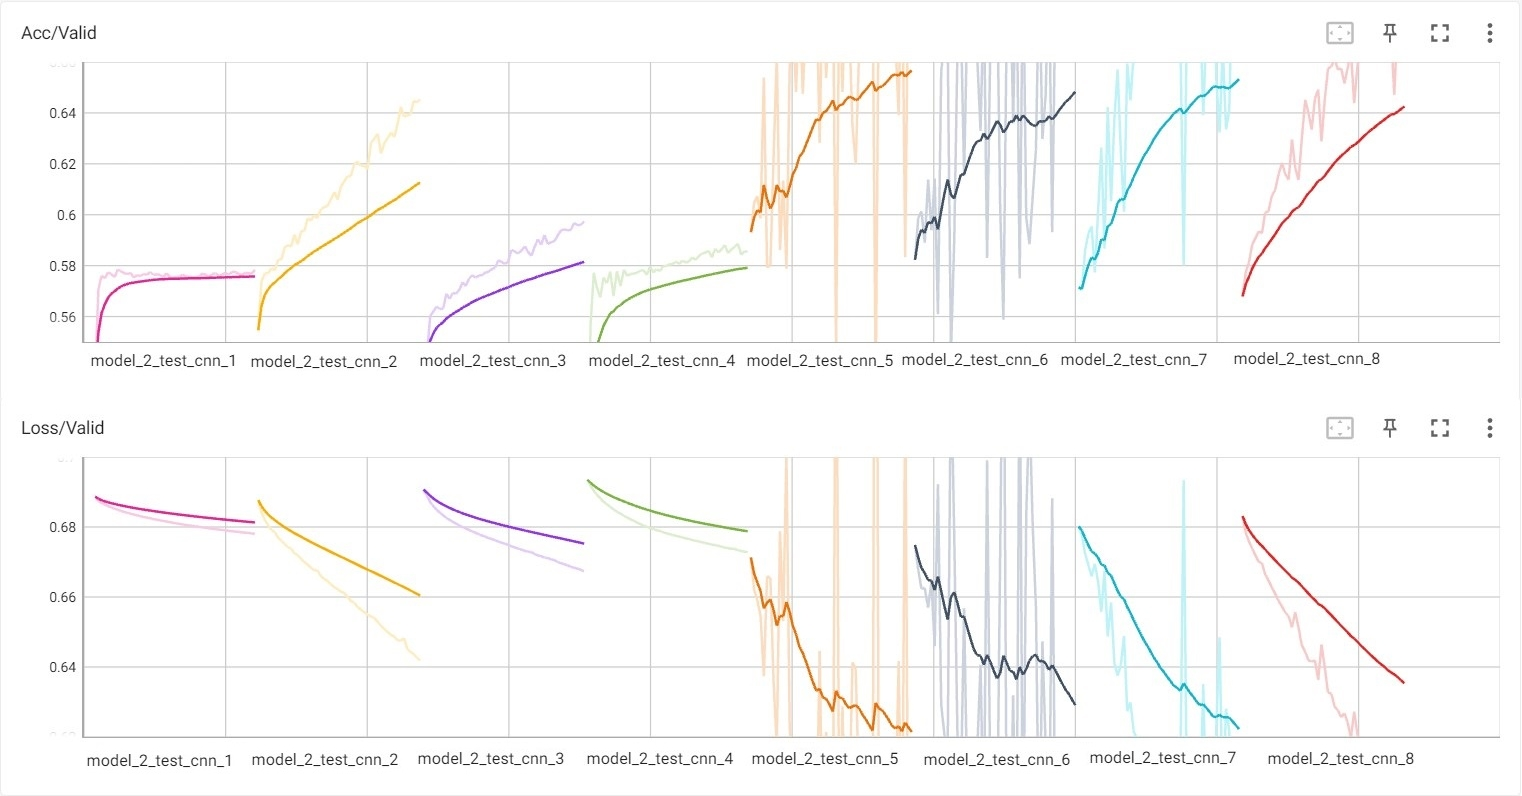
\includegraphics[width=\textwidth]{img/exp1_acc2+loss2.jpg}
        \label{fig:exp1_mod2}
        \caption{Experiment 1 - Results for Model 2}
    \end{figure}
\end{center}

\end{frame}



\begin{frame}{Technical implementation}{Experiment 1}

\begin{center}
    \begin{figure}[!h]
        \centering
        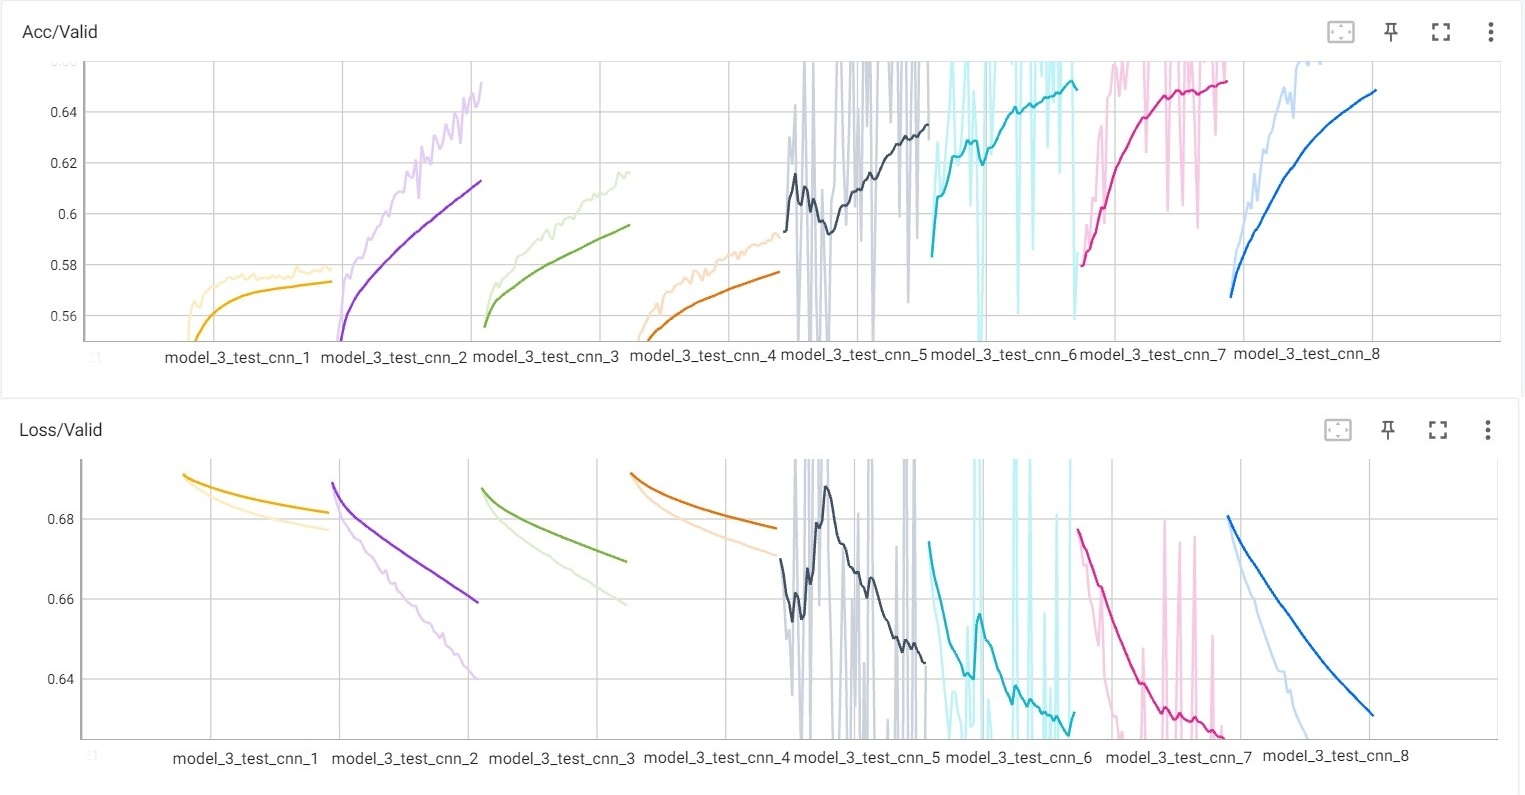
\includegraphics[width=\textwidth]{img/exp1_acc3+loss3.jpg}
        \label{fig:exp1_mod3}
        \caption{Experiment 1 - Results for Model 3}
    \end{figure}
\end{center}

\end{frame}



\begin{frame}{Technical implementation}{Experiment 1}

\begin{center}
    \begin{figure}[!h]
        \centering
        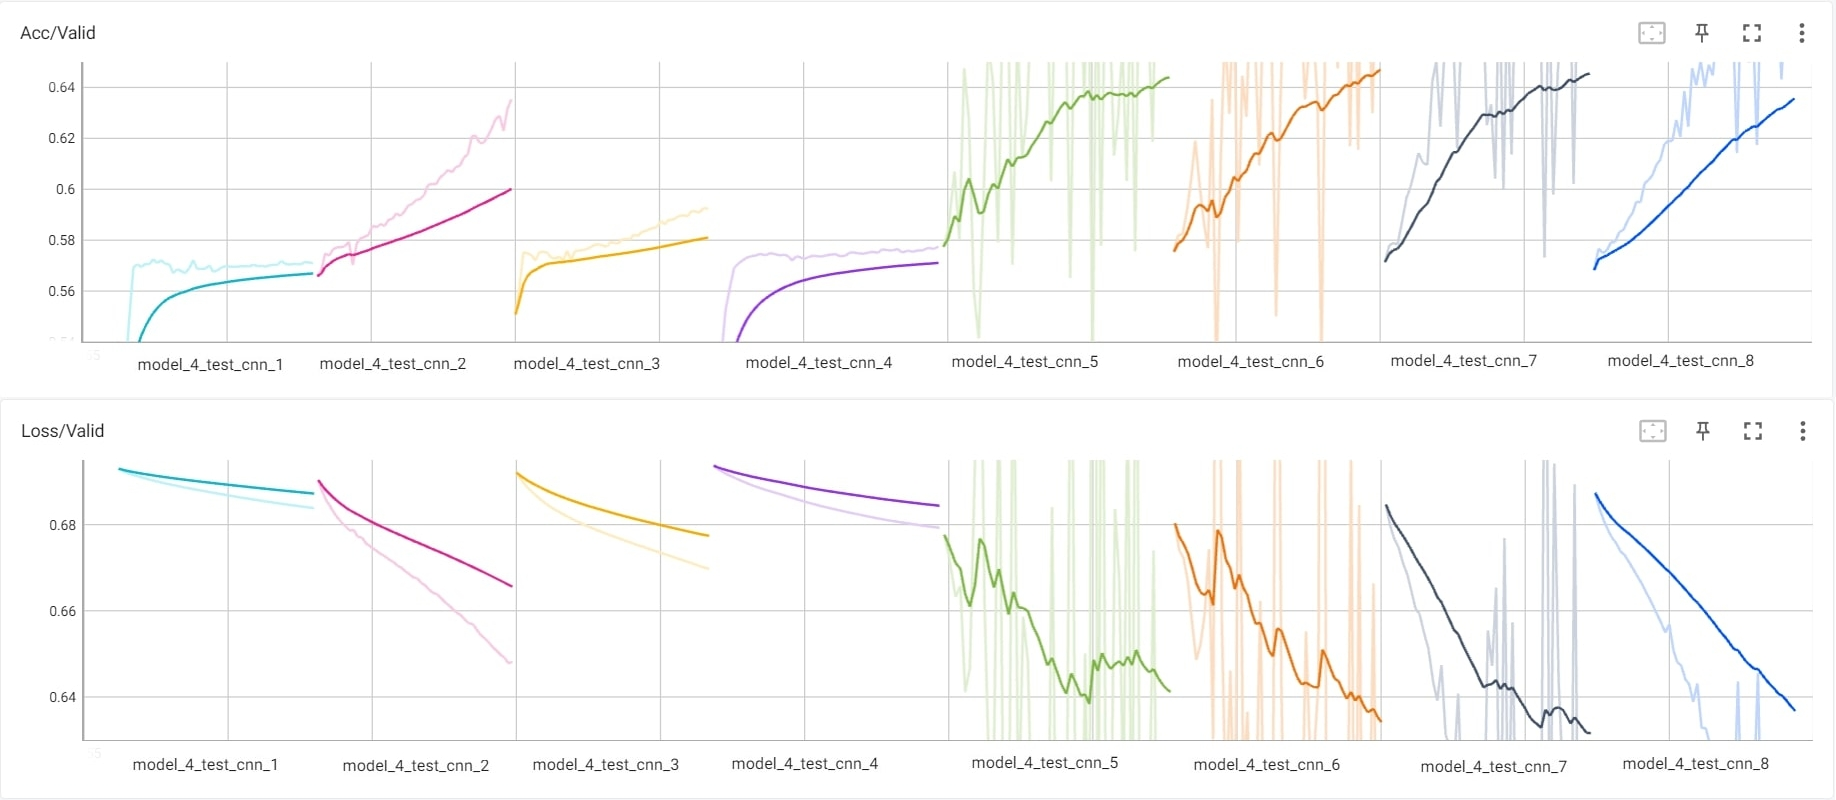
\includegraphics[width=\textwidth]{img/exp1_acc4+loss4.jpg}
        \label{fig:exp1_mod4}
        \caption{Experiment 1 - Results for Model 4}
    \end{figure}
\end{center}

\end{frame}



\begin{frame}{Technical implementation}{Experiment 1}

\begin{center}
    \begin{figure}[!h]
        \centering
        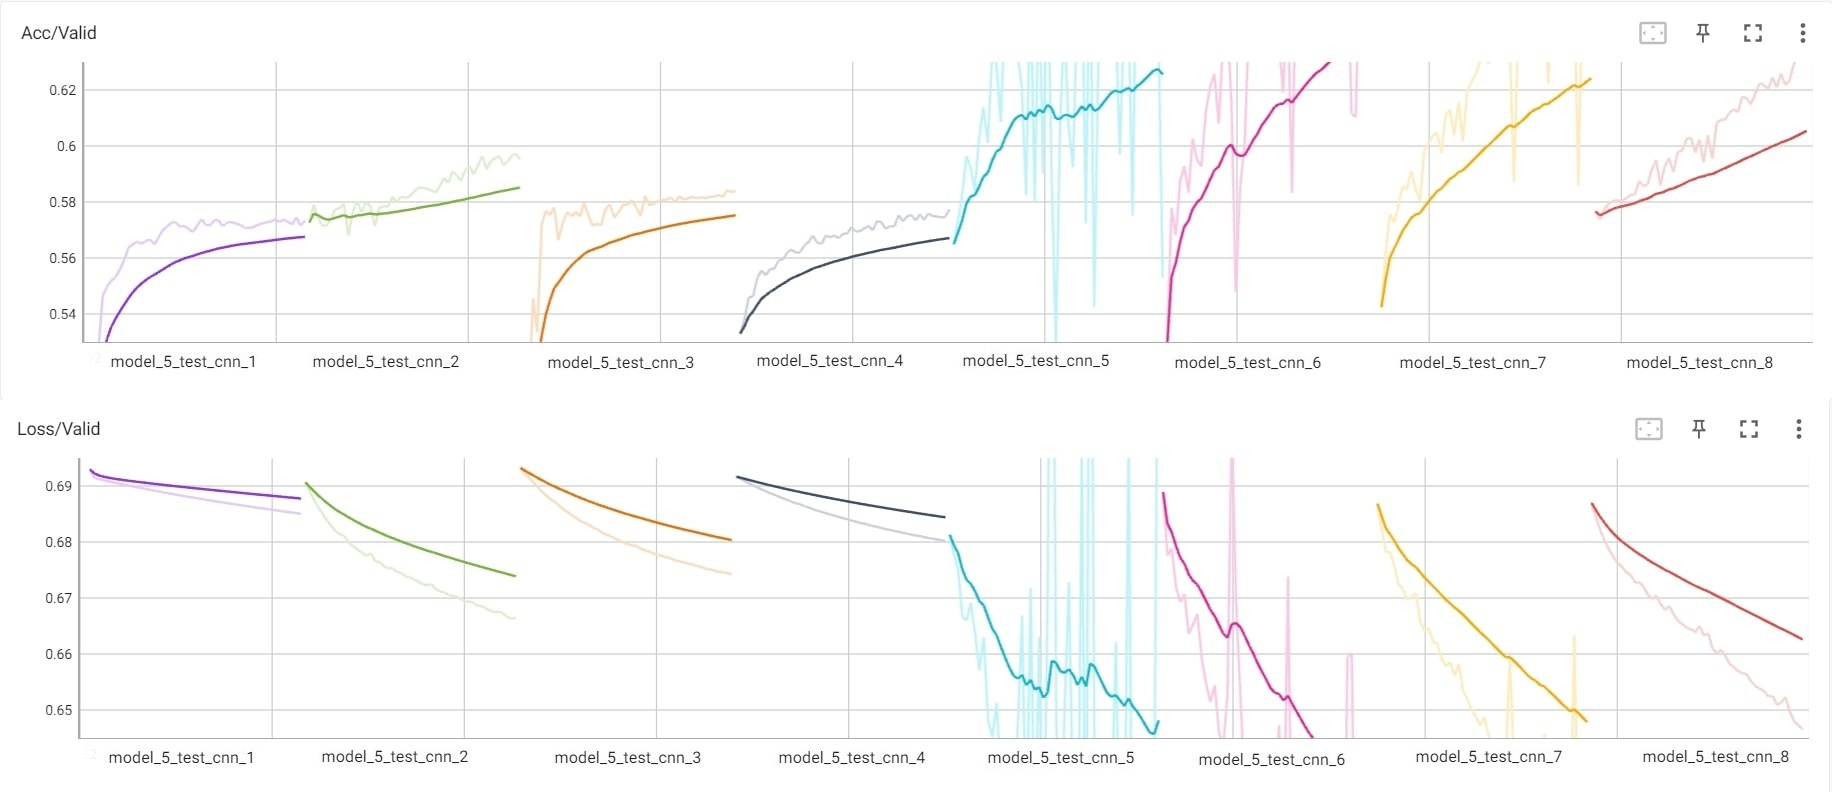
\includegraphics[width=\textwidth]{img/exp1_acc5+loss5.jpg}
        \label{fig:exp1_mod5}
        \caption{Experiment 1 - Results for Model 5}
    \end{figure}
\end{center}

\end{frame}


\begin{frame}{Technical implementation}{Experiment 1}

\begin{center}
    \begin{figure}[!h]
        \centering
        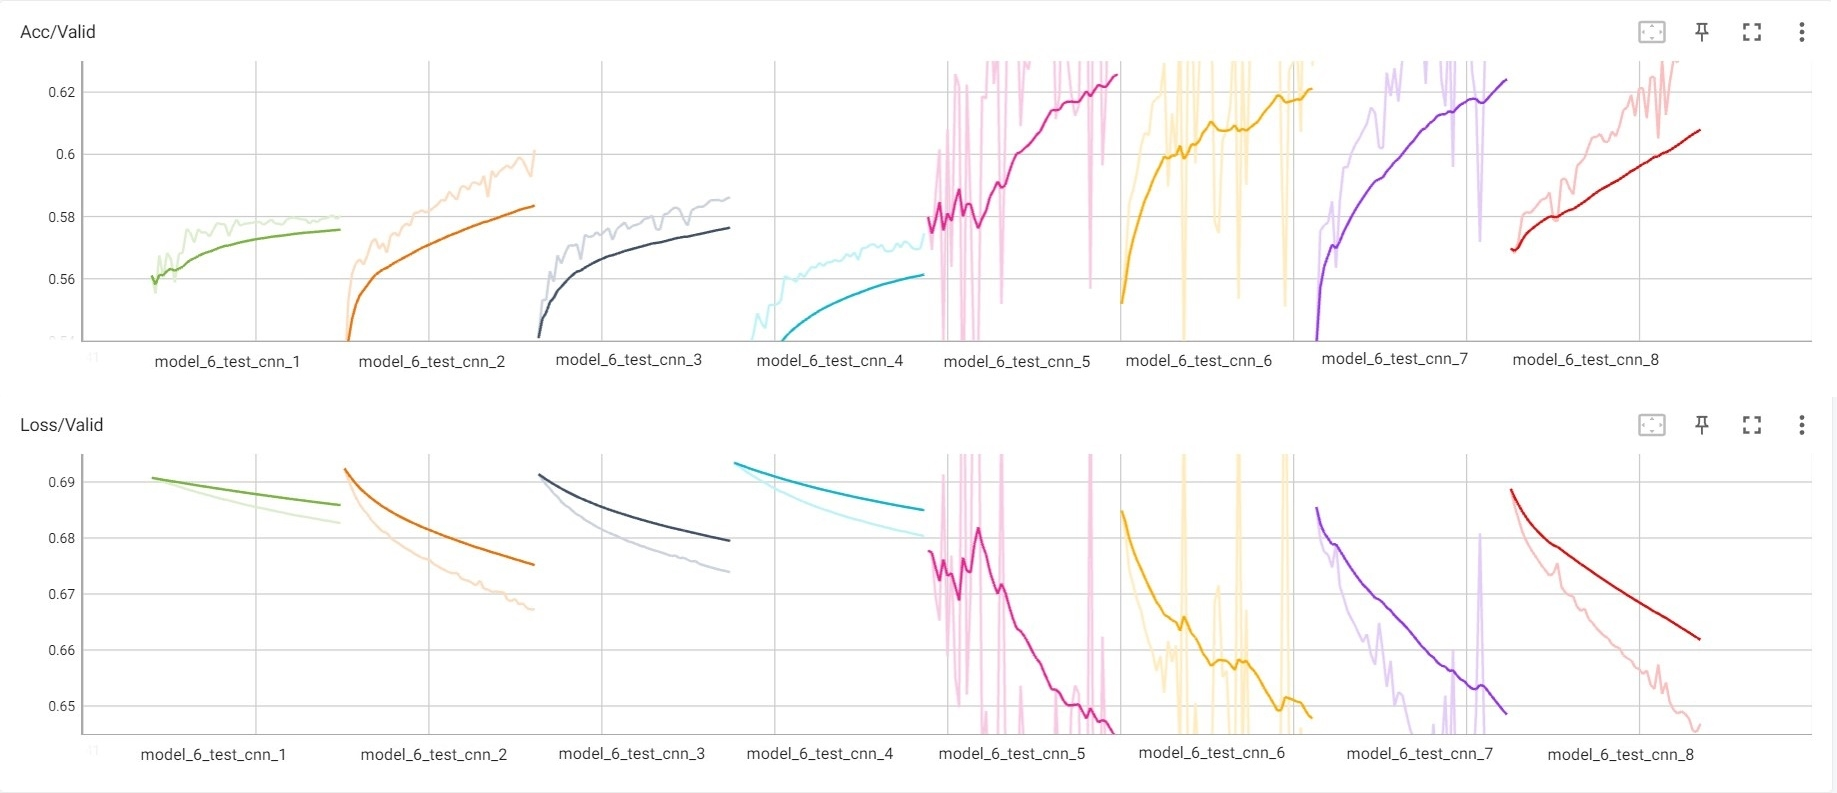
\includegraphics[width=\textwidth]{img/exp1_acc6+loss6.jpg}
        \label{fig:exp1_mod6}
        \caption{Experiment 1 - Results for Model 6}
    \end{figure}
\end{center}

\end{frame}








\begin{frame}{Technical implementation}{Experiment 2}

\hspace{0.4cm}  As already noticed, models 2, 3 and 4 had high accuracy, so we will use them to do fine tuning when we retrain the BERT model as well. The learning rate took the values: $4*10^{-5}, 2*10^{-5}$. The batch size was kept at 32.

\begin{center}
    \begin{figure}[!h]
        \centering
        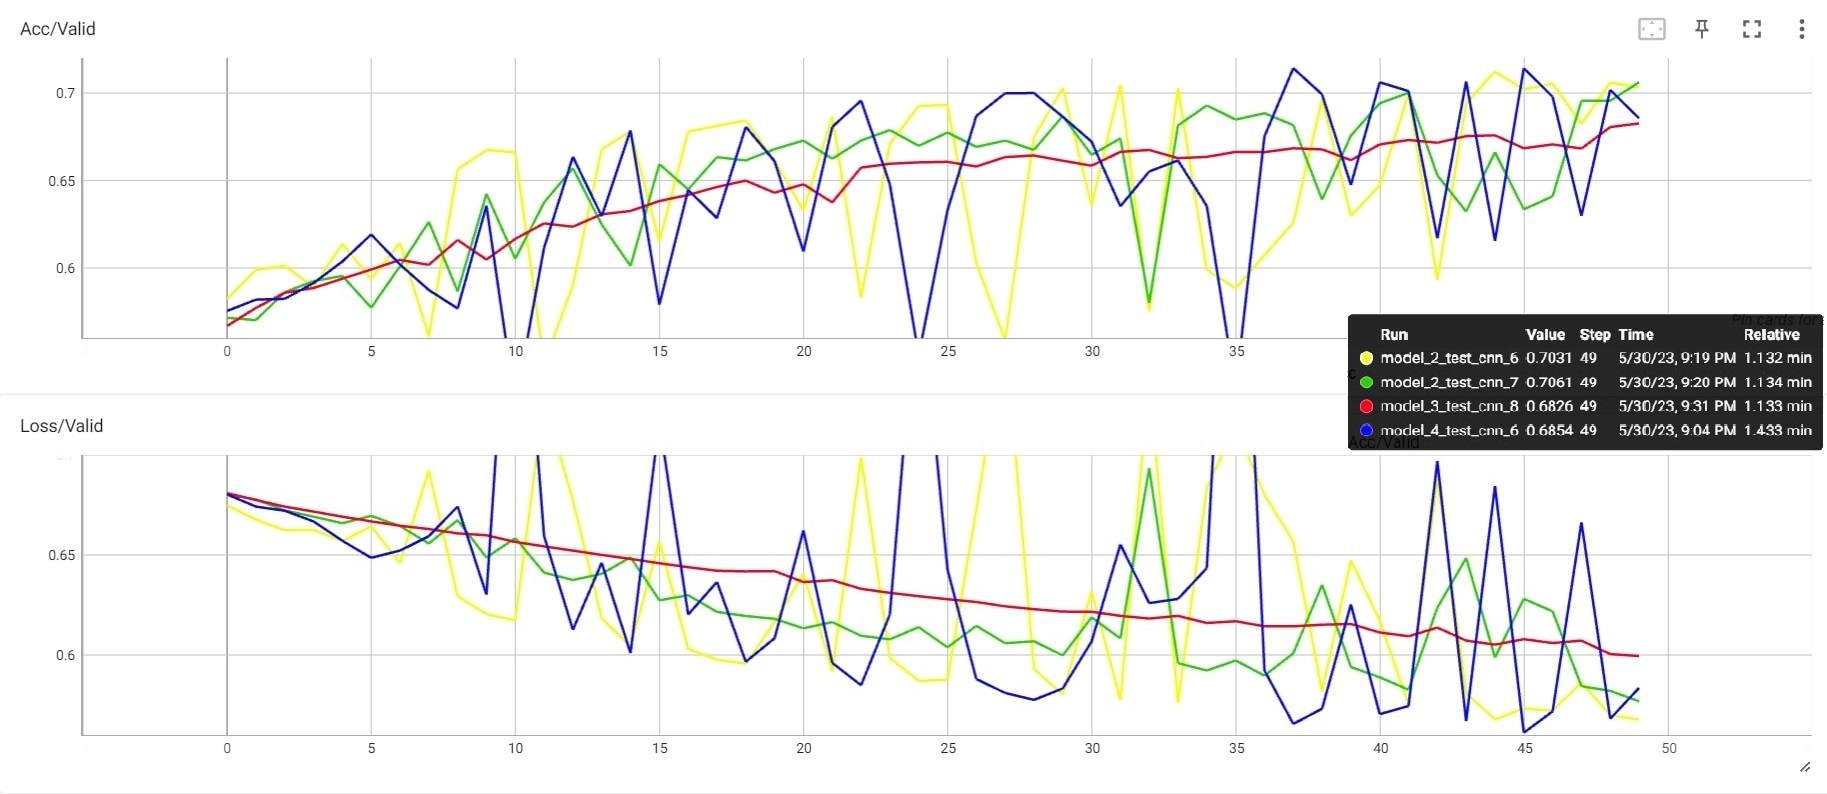
\includegraphics[width=0.8\textwidth]{img/exp1_hiperparametrizare.jpg}
        \label{fig:exp1_hiperm}
        \caption{Experiment 1 - Results for Model 2, 3 and 4}
    \end{figure}
\end{center}

\end{frame}



\begin{frame}{Technical implementation}{Experiment 2}

\begin{center}
    \begin{figure}[!h]
        \centering
        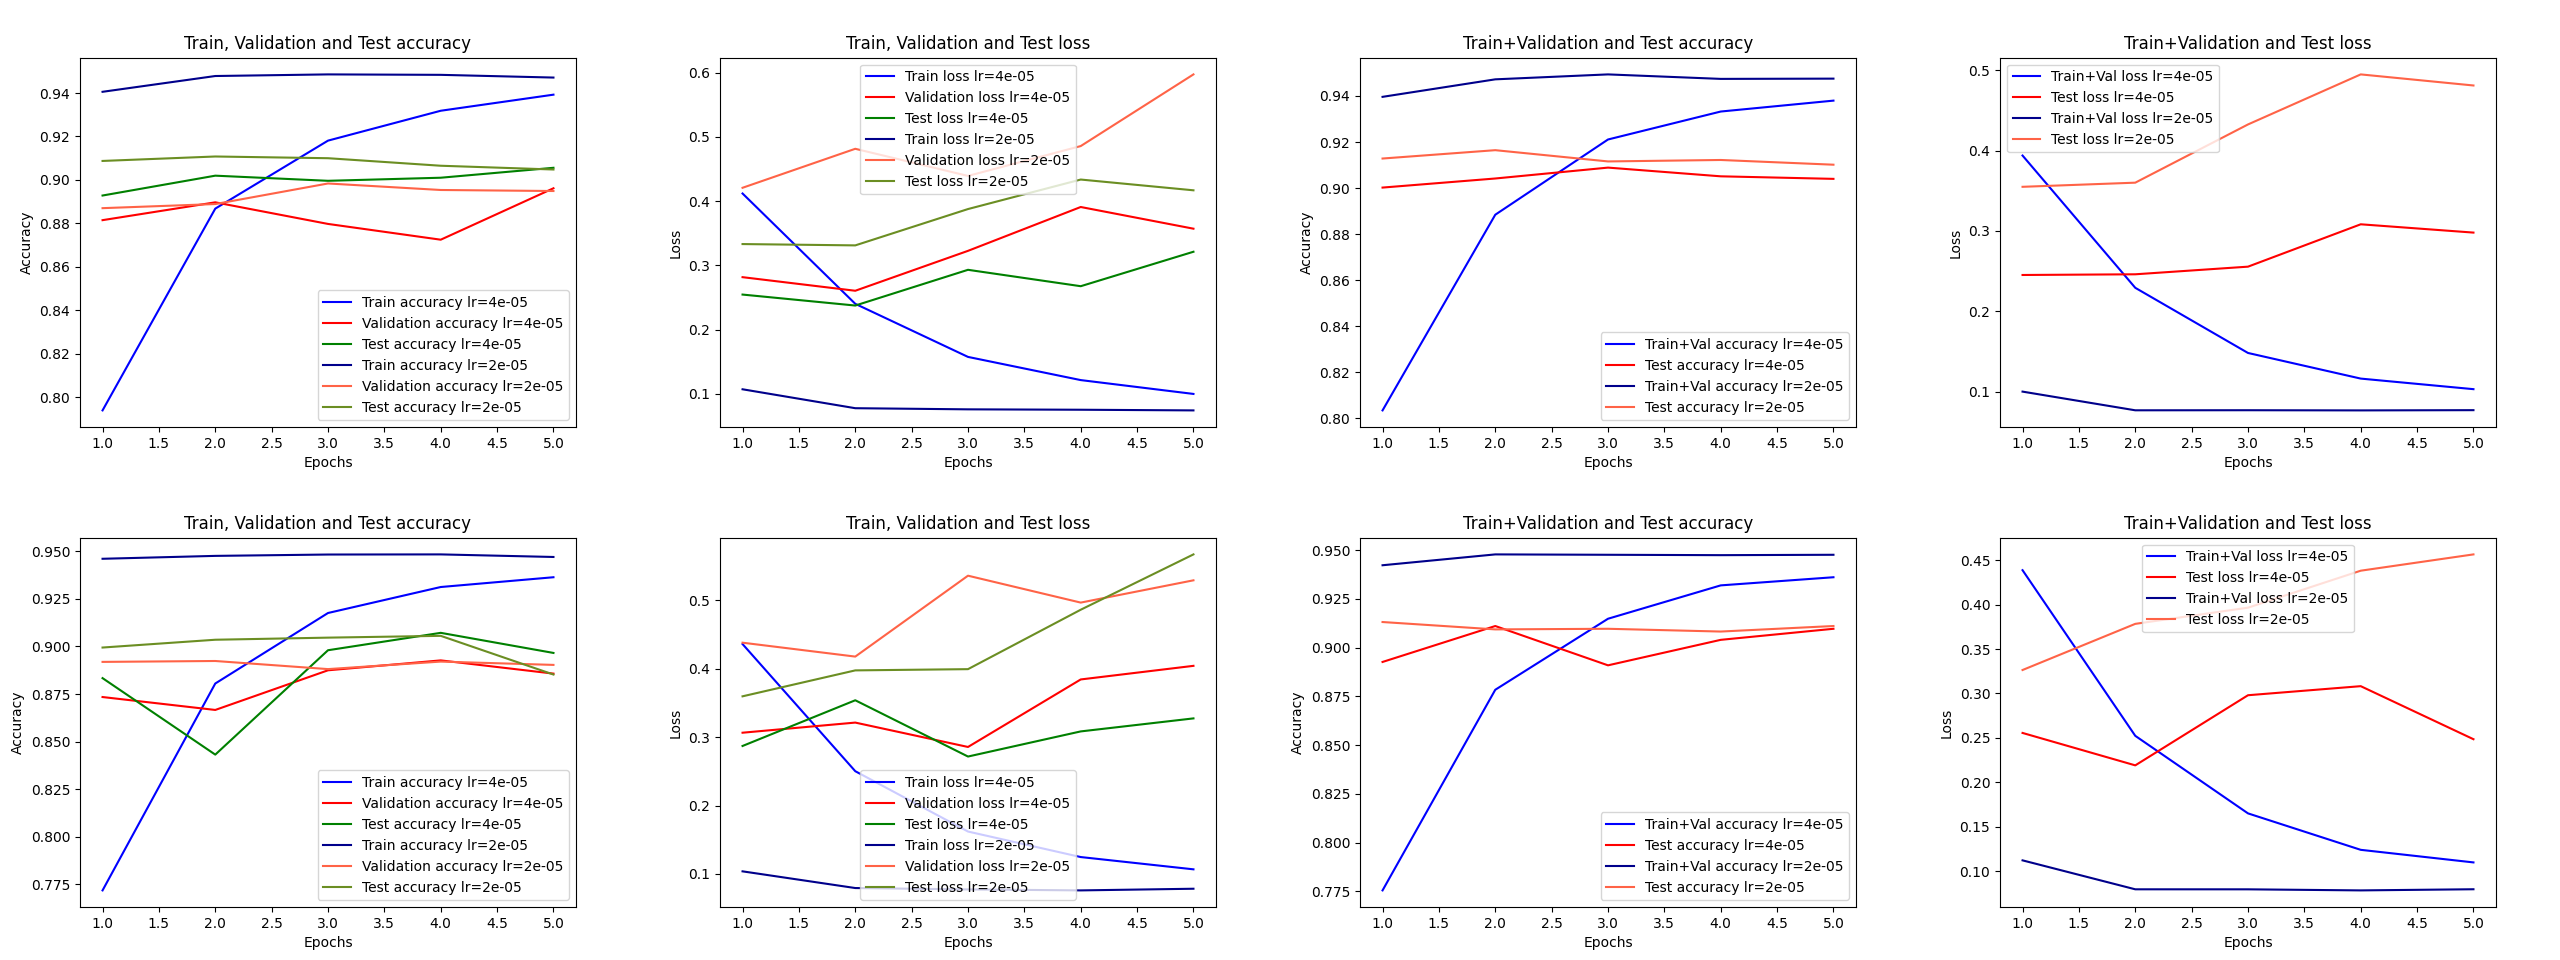
\includegraphics[width=\textwidth]{img/ger_model1.png}
        \label{fig:ger_model1}
        \caption{Results for Model 2 with and without BERT activation. Tested on Validation(left) and on Test(right)}
    \end{figure}
\end{center}

\end{frame}



\begin{frame}{Technical implementation}{Experiment 2}

\begin{center}
    \begin{figure}[!h]
        \centering
        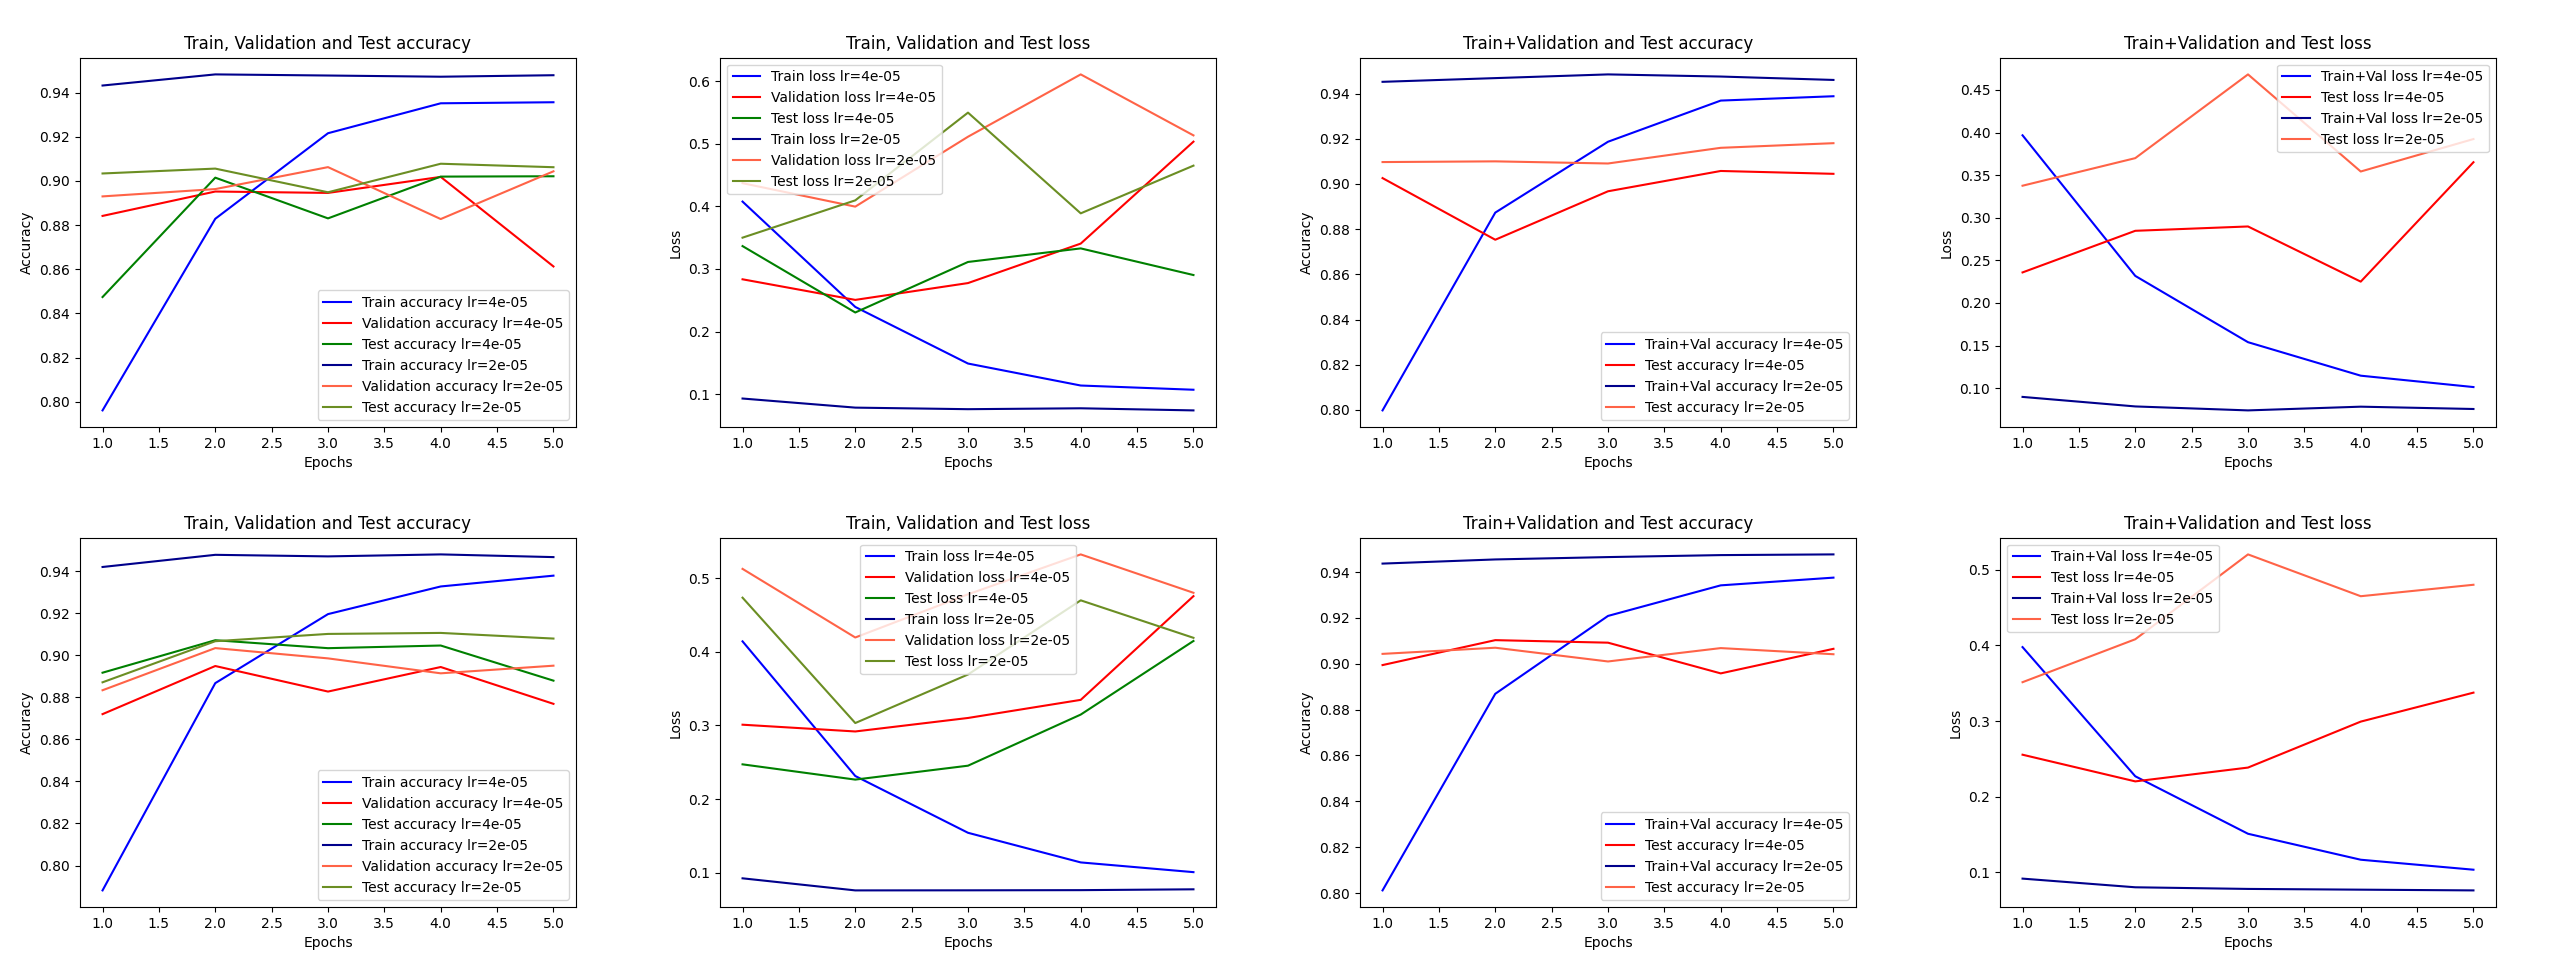
\includegraphics[width=\textwidth]{img/ger_model2.png}
        \label{fig:ger_model2}
        \caption{Results for Model 3 with and without BERT activation. Tested on Validation(left) and on Test(right)}
    \end{figure}
\end{center}

\end{frame}


\begin{frame}{Technical implementation}{Experiment 2}

\begin{center}
    \begin{figure}[!h]
        \centering
        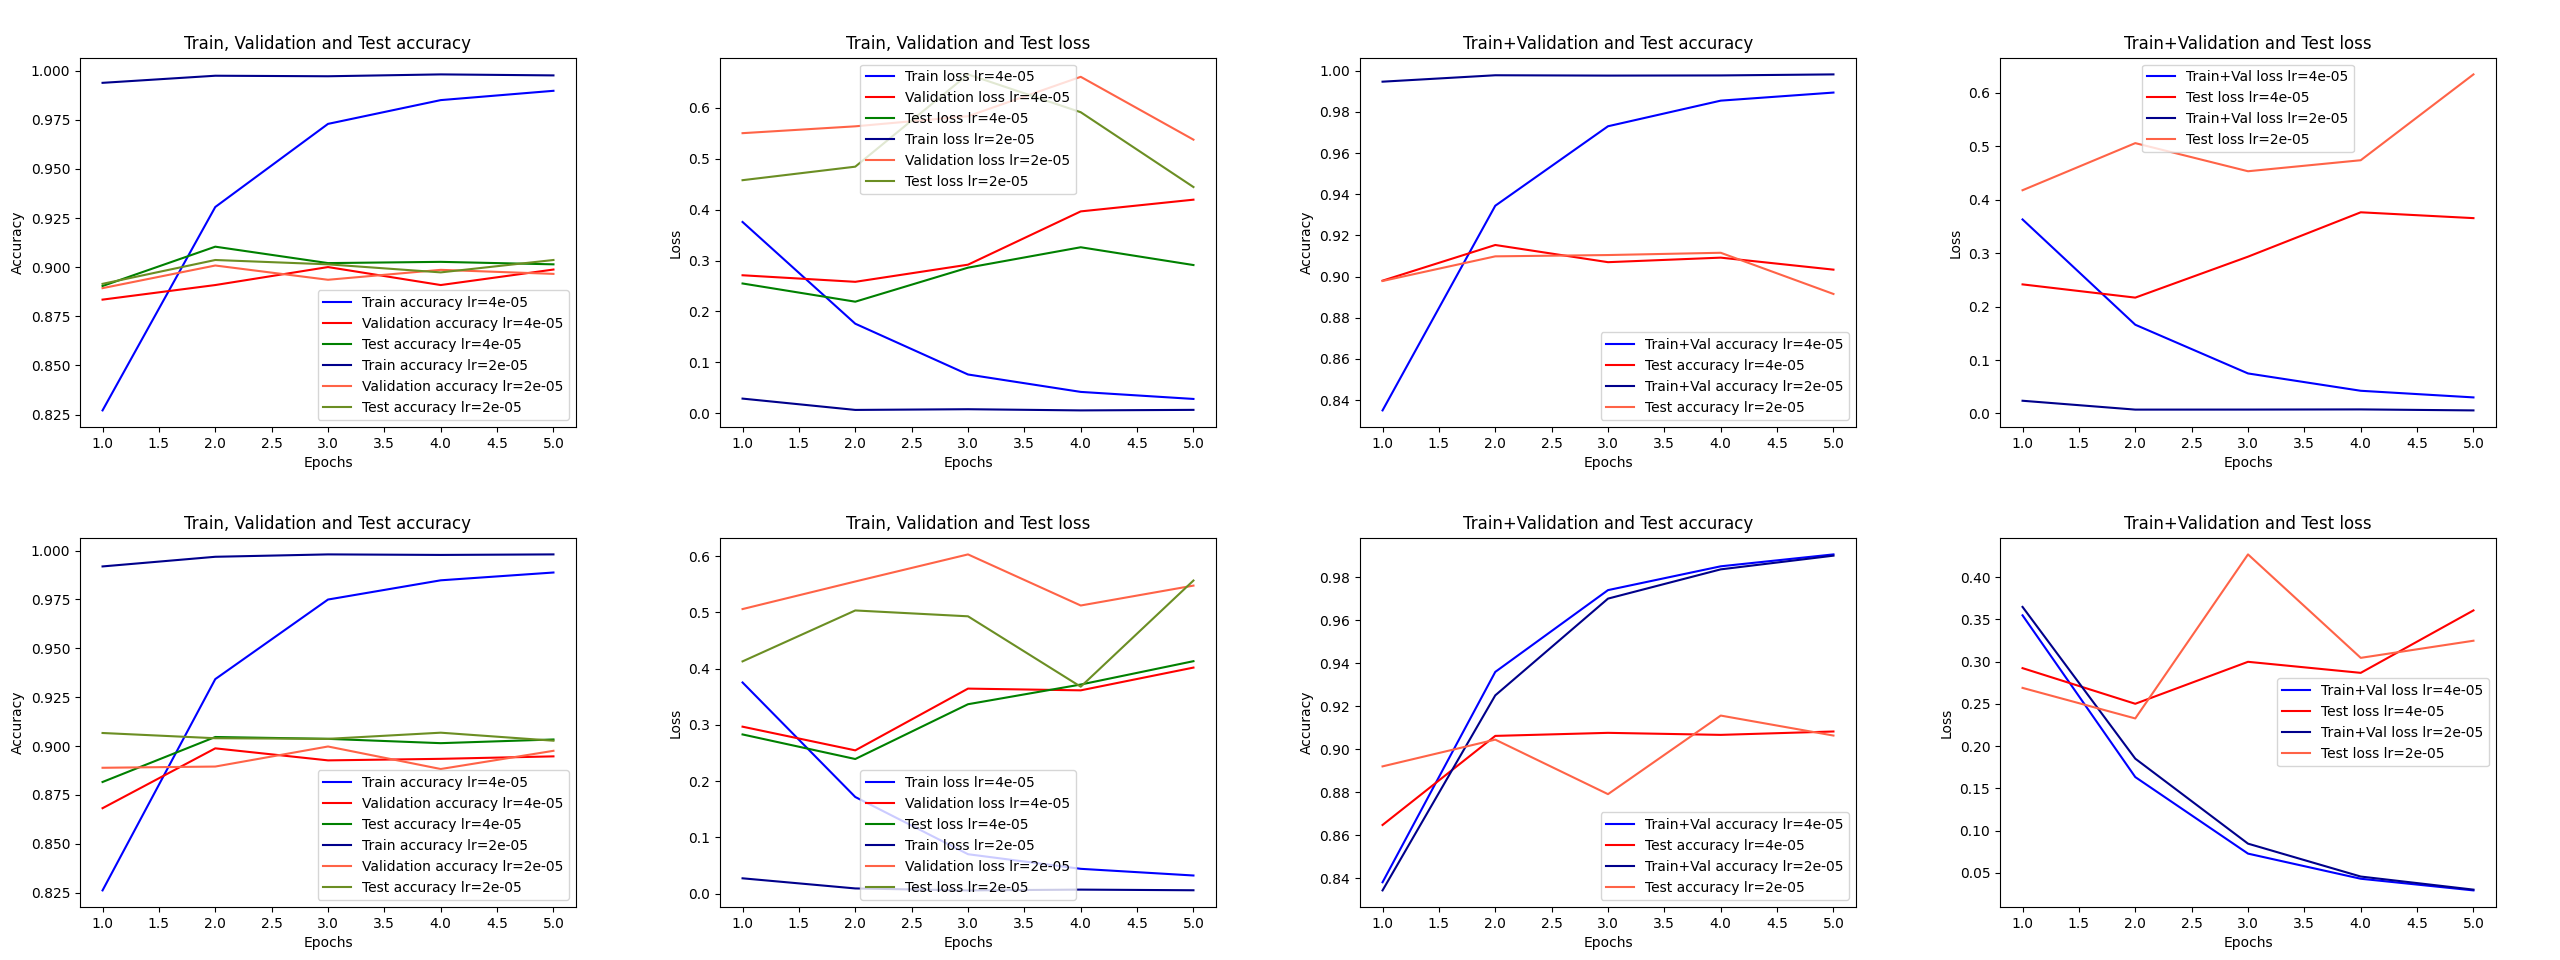
\includegraphics[width=\textwidth]{img/ger_model3.png}
        \label{fig:ger_model3}
        \caption{Results for Model 4 with and without BERT activation. Tested on Validation(left) and on Test(right)}
    \end{figure}
\end{center}

\end{frame}



\section[Results]{Results}

\begin{frame}{Results}{Experiment 1}

\begin{center}
    \begin{tabular}{|p{3cm}||p{3cm}|p{3cm}|  }
     % \hline
     % \multicolumn{3}{|c|}{BERT fine-tunning results} \\
     \hline
    Model number	& Accuracy & Loss \\
     \hline
    Model 1 & 71.07\% & 0.5611\\
    \textbf{Model 2} & \textbf{71.23}\% & 0.5691\\
    \textbf{Model 3} & \textbf{71.4}\% & 0.5682\\
    \textbf{Model 4} & \textbf{71.42}\% & 0.5611\\
    Model 5 & 68.58\% & 0.5994\\
    Model 6 & 69.03\% & 0.6034\\
     \hline
    \end{tabular}
    \captionof{table}{BERT fine-tunning results: Experiment 1}
\end{center}

\end{frame}



\begin{frame}{Results}{Experiment 2}

\begin{table}
\scriptsize
    \begin{tabular}{|p{2.0cm}||p{2.0cm}|p{2.0cm}|p{2.0cm}|p{2.0cm}|  }
     \hline
    Model no.& Acc on Train	& Loss on Train & Acc on Test & Loss on Test\\
     \hline
     \multicolumn{5}{|c|}{DE-EN dataset} \\
     \hline
    Model 2-A&  94.935\%  &  0.103  &  91.646\%  &  0.36 \\
    Model 2-B&  94.785\%  &  0.11  &  91.315\%  &  0.326 \\
    Model 3-A&  94.846\%  &  0.101  &  91.803\%  &  0.392 \\
    Model 3-B&  94.771\%  &  0.103  &  91.031\%  &  0.408 \\
    Model 4-A&  99.825\%  &  0.03  &  91.535\%  &  0.474 \\
    Model 4-B&  99.067\%  &  0.03  &  91.567\%  &  0.361 \\
     \hline
     \multicolumn{5}{|c|}{ES-EN dataset} \\
     \hline
    Model 2-A&  95.097\%  &  0.102  &  91.992\%  &  0.325 \\
    Model 2-B&  95.005\%  &  0.1  &  92.04\%  &  0.384 \\
    Model 3-A&  94.963\%  &  0.102  &  92.055\%  &  0.409 \\
    Model 3-B&  94.944\%  &  0.099  &  92.323\%  &  0.365 \\
    Model 4-A&  99.833\%  &  0.03  &  91.992\%  &  0.404 \\
    Model 4-B&  99.805\%  &  0.028  &  92.229\%  &  0.358 \\
     \hline
     \multicolumn{5}{|c|}{A: BERT not activated, B: BERT activated} \\
     \hline
    \end{tabular}
    \captionof{table}{BERT results: Experiment 2}
\end{table}

\end{frame}


\begin{frame}{Results}{Compared results}

\begin{table}
    \begin{tabular}{|p{2.5cm}||p{2.5cm}|p{2.5cm}|  }
     \hline
    Dataset	& Model & Accuracy \\
     \hline
     \hline
    DE-EN&  $BERT^{*}$  &  \textbf{92.4}\%\\
    DE-EN&  Model 3-A  &  91.8\%  \\
    \hline
    \hline
    ES-EN&  $BERT^{*}$  &  91.4\%\\
    ES-EN&  Model 3-B  &  \textbf{92.32}\%  \\
     \hline
     \multicolumn{3}{|c|}{$BERT^{*}$: BERT best result from paper \cite{mainpaper}} \\
     \hline
    \end{tabular}
    \captionof{table}{Compared results}
\end{table}


\end{frame}


% \section[Constraints]{Constraints}
% \begin{frame}{Constraints}

% \begin{itemize}
%     \item the reliance on pre-existing large language models
%     \item requirement for extensive computational resources
% \end{itemize}

% \end{frame}


\section[Practic Applications of our model]{Practic Applications of our model}

\begin{frame}{Practic Applications of our model}

\hspace{0.4cm} The findings from this study have several practical applications that can benefit various stakeholders in the field of translation and language processing. Here are some practical applications of a BERT model trained to detect English translationese classification based on the research:
\begin{itemize}
    \item Translation Quality Assessment: as an objective tool for translated-text quality assessment
    \item Translator Training and Feedback: as an educational tool for translator training programs
    \item Translation Memory Optimization: can receive suggestions or warnings when translationese patterns are detected in segments
    \item Machine Translation Improvement: can be integrated into machine translation(MT) systems to enhance their output quality
\end{itemize}

\end{frame}




\section[Future Research Directions]{Future Research Directions}

\begin{frame}{Future Research Directions}

\begin{itemize}
    \item Cross-Linguistic Analysis: Extending the study to include a broader range of languages and language pairs can help uncover language-specific characteristics and identify common translationese patterns across different linguistic backgrounds.
    
    \item Addressing Ethical Concerns: As LLMs continue to grow and expand, ethical considerations become crucial. Future research should tackle diagnosis bias worries, fairness, and more importantly, transparency in translationese classification to ensure responsible and equitable use of these models.

    \item Using bigger models: For example, this paper is used bert-base-uncased which has 110M parameters. For future work, we may want to use bert-large-uncased which has 340M parameters and may be better to classify translationese
\end{itemize}

\end{frame}



\section[Conclusion]{Conclusion}

\begin{frame}{Conclusion}

\hspace{0.4cm} By pursuing these future research directions, the field of translation studies can further leverage the capabilities of large language models and advance our  extended comprehension of translationese, ultimately benefiting translation professionals and improving cross-linguistic communication.

\end{frame}

\nocite{*}
\section{\bibname}
\begin{frame}[t, allowframebreaks]{\bibname}
\printbibliography[heading=none]
\end{frame}


\begin{frame}%[plain]
\vfill
\centerline{Thank You for Your Attention!}
\vfill\vfill
\end{frame}
%\input{sample}

\end{document}


